\documentclass[10pt,a4paper, nocenter]{beamer}
\usetheme{AnnArbor}
\usecolortheme{seahorse}
\usepackage[scaled=0.92]{helvet}
\usepackage[latin1]{inputenc}
\usepackage{blindtext}
\usepackage{amsmath}
\usepackage{appendix}
\usepackage{amsfonts}
\usepackage{amssymb,amsthm}
\usepackage{graphicx}
\usepackage{parskip}
\usepackage{fancyhdr}
\usepackage{lastpage}
\usepackage{enumerate,url}
\usepackage{etoolbox}
\usepackage{algorithm2e}
\usepackage{caption}
\usepackage{subcaption}

\author[S. Antani (supervisor Dr. Zhou)]{Sourabh Antani \\ supervisor \\ Dr. Yunkai Zhou}
\title[Spectral Clustering]{Research Report - Spectral Clustering}
\date{June 3, 2021}
\institute[SMU - MATH]{Mathematics Department,\\Southern Methodist University}
\begin{document}
	\begin{frame}
		\titlepage
	\end{frame}
    
    \begin{frame}
    \section{Clustering Algorithms}
    \frametitle{Clustering Algorithms}
    Below are some examples of clustering algorithms used in practice, aside from spectral clustering. 
    \begin{itemize}
        \item <1-> Euclidean distance and spatial density based:
	    \begin{itemize}
    	    \item <2-> $k$-means [Macqueen, 1967] [Lloyd 1982]
            \item <3-> BIRCH (Balanced Iterative Reducing and Clustering using Hierarchies) [Zhang et al. 1996]
            \item <4-> Mean-shift [Cheng 1995]
            \item <5-> DBSCAN [Ester et al. 1996]
		\end{itemize}
        \item <6-> Linear Algebra based
	    \begin{itemize}
	    	\item <7-> Non-Negative Matrix Factorization [Lawton et al. 1971] [Paatero et al. 1991] [Ding et al. 2005]
            \item <8-> PCA Based clustering [Zhang et al. 2018]
        \end{itemize}
    \end{itemize}
    \end{frame}

	
	\begin{frame}{Spectral Clustering}
		\framesubtitle{Graph Laplacian - Construction}
		
		\begin{itemize}
			\item<1-> Given an undirected graph, $\mathbf{G=(V,E)}$ with set of vertices $\mathbf{V=\{v_{1},\dots,v_{n}\}}$ and $\mathbf{E}$ set of weighted edges. The weight of the edge between $v_i$ and $v_j$, denoted by $w_{ij}$ is assigned based on the 'similarity' between the data-points $v_i$ and $v_j$. For example, if the similarity function chosen is a Gaussian kernel and the data that these vertices represent are scalars $x_i$ and $x_j$, then $w_{ij} = e^{-\lvert x_i - x_j \rvert^2/2}$
			\item<2-> Construct the Weighted adjacency matrix $\mathbf{W=(w_{ij})_{i,j=1,\dots,n}}$ and Degree matrix $\mathbf{D} = diag(d_{1} ,\dots, d_{n})$ where $\mathbf{d_{i} = \sum_{j=1}^{n}w_{ij}}$ is called Degree of a vertex $v_i$.
			\item<3-> Graph Laplacian is defined as $L = D - W$
			\item<4-> A fully connected graph can be made sparse by converting it into a $k$-nearest neighbor or an $\epsilon$-neighborhood graph.
		\end{itemize}
	\end{frame}


	\begin{frame}{Spectral Clustering}
		\framesubtitle{Graph Laplacian - Types and Properties [Luxburg, 2007]}
		
		\begin{itemize}
			\item<1-> Unnormalized Graph Laplacian [Mohar, 1991], [Mohar, 1997]
				\begin{itemize}
					\item $L = D-W$ (Symmetric)
				\end{itemize}
			\item<2-> Normalized Symmetric Graph Laplacian [Chung, 1997]
				\begin{itemize}
					\item $L_{sym} = D^{-1/2}LD^{-1/2} = I - D^{-1/2}WD^{-1/2}$ (Symmetric)
				\end{itemize}
			\item<3-> Normalized Random Walk Graph Laplacian [Chung 1997]
				\begin{itemize}
					\item $L_{rw} = D^{-1}L = I - D^{-1}W$ (Not-Symmetric)
				\end{itemize}
			\item<4-> The eigenpair $(\lambda, u)$ of $L_{rw}$ solve $Lu=\lambda Du$ and in this case $D^{1/2}u$ is eigenvector of $L_{sym}$ with eigenvalue $\lambda$. 
			\item<5-> All Laplacians are Positive-semidefinte, hence have non-Negative Real-Valued Eigenvalues
			\item<6-> 0 is an eigenvalue with multiplicity equal to number of connected components
		\end{itemize}
	\end{frame}

	\begin{frame}{Spectral Clustering}
		\framesubtitle{Graph Cuts}
		\begin{itemize}
			\item<1-> The goal of clustering is to maximize the similarity within cluster and minimize the similarity between clusters.
			\item<2-> Minimizing the between cluster similarity equals to minimizing the objective function $$  \text{cut}(A_{1}, \dots, A_{k}) := \frac{1}{2}\sum_{i-1}^{k}W(A_i,\bar{A}_{i}),\hspace{10pt} \text{where }W(A,B) = \sum_{i\in A, j\in B}w_{ij}, \bar{A} = V \backslash A $$
			\item<3-> To maximize the within-cluster similarity, we define two objective functions \begin{align*} RatioCut(A_{1},\dots,A_{k}) &= \frac{1}{2} \sum_{i=1}^{k}\frac{W(A_{i},\bar{A}_{i})}{\lvert A_{i} \rvert}
				= \sum_{i=1}^{k}\frac{cut(A_{i},\bar{A}_{i})}{\lvert A_{i} \rvert} [Hagen, Kahng,  1992]\\
				Ncut(A_{1},\dots,A_{k}) &= \frac{1}{2}\sum_{i=1}^{k}\frac{W(A_{i},\bar{A}_{i})}{vol(A_{i})} = 
				\sum_{i=1}^{k}\frac{cut(A_{i},\bar{A}_{i})}{vol(A_{i})} [Shi, Malik, 2000]\\
			\end{align*}
			
		\end{itemize}
	\end{frame}

	\begin{frame}{Spectral Clustering}
		\framesubtitle{Algorithms - Unnormalized Spectral Clustering - Hagen \& Kahng (1992)}
		\begin{algorithm}[H]
			\DontPrintSemicolon
			\KwIn{Similarity matrix $S \in \mathbb{R}^{n\times n}$, number $k$ of clusters to construct.}
			\Begin{
				Construct a similarity graph and its weighted adjacency matrix $W$ according to the chosen similarity function\;
				Compute the unnormalized Laplacian $L$\;
				Compute the first $k$ eigenvectors $u_{1},\dots, u_{k} $ of $L$\;
				Let $U \in \mathbb{R}^{n\times k}$ be the matrix containing the vectors $u_{1}, \dots , u_{k}$ as columns\;
				For $i = 1,\dots, n$, let $y_{i} \in \mathbb{R}^k$ be the vector corresponding to the $i^{th}$ row of $U$\;
				Cluster the points $(y_{i}), i=1,\dots,n$ in $\mathbb{R}^k$ with the k-means algorithm into clusters $C_{1},\dots, C_{k}$\;}
			\KwOut{Clusters $A_{1},\dots, A_{k}$ with $A_{i} = \{x_{j}| y_{j} \in C_{i}\}$}
		\end{algorithm}		
	\end{frame}

		\begin{frame}{Spectral Clustering}
		\framesubtitle{Algorithms - Normalized Spectral Clustering - Shi \& Malik (2000) }
		\textit{This algorithm uses generalized eigenvectors of L, which are the eigenvectors of normalized random-walk Laplacian $L_{rw}= D^{-1}L$}
		\begin{algorithm}[H]
			\DontPrintSemicolon
			\KwIn{Similarity matrix $S \in \mathbb{R}^{n\times n}$, number $k$ of clusters to construct}
			\Begin{
				Construct a similarity graph and its weighted adjacency matrix $W$ according to the chosen similarity function\;
				Compute the unnormalized Laplacian $L$.\;
				Compute the first $k$ generalized eigenvectors $u_{1},\dots, u_{k} $ of generalized eigenproblem $Lu = \lambda Du$.\;
				Let $U \in \mathbb{R}^{n\times k}$ be the matrix containing the vectors $u_{1},\dots , u_{k}$ as columns.\;
				For $i = 1,\dots, n$, let $y_{i} \in \mathbb{R}^k$ be the vector corresponding to the $i^{th}$ row of $U$.\;
				Cluster the points $(y_{i}), i=1,\dots ,n$ in $\mathbb{R}^k$ with the k-means algorithm into clusters $C_{1},\dots , C_{k}$.\;
			}
			\KwOut{Clusters $A_{1},\dots, A_{k}$ with $A_{i} = \{x_{j}| y_{j} \in C_{i}\}$}
		\end{algorithm}
		
	\end{frame}
	
	\begin{frame}{Spectral Clustering}
		\framesubtitle{Algorithms - Normalized Spectral Clustering - Ng, Jordan \& Weiss (2002) }
		\textit{This algorithm uses the eigenvectors of normalized symmetric Laplacian $L_{sym} = D^{-1/2}LD^{-1/2}$. Note that if $D^{1/2}u$ is an eigenvector of $L_{sym}$ if $u$ is an eigenvector of $L$ hence an additional normalization step is needed.}
		
		\begin{algorithm}[H]
			\DontPrintSemicolon
			\KwIn{Similarity matrix $S \in \mathbb{R}^{n\times n}$, number $k$ of clusters to construct.}
			\Begin{
				Construct a similarity graph and its weighted adjacency matrix $W$ according to the chosen similarity function\;
				Compute the normalized Laplacian $L_{sym}$\;
				Compute the first $k$ eigenvectors $u_{1},\dots, u_{k} $ of $L_{sym}$\;
				Let $U \in \mathbb{R}^{n\times k}$ be the matrix containing the vectors $u_{1},\dots, u_{k}$ as columns\;
				Form the matrix $T \in \mathbb{R}^{n\times k}$ from $U$ by normalizing the norm to 1, $t_{ij} = u_{ij}/(\sum_{k}u_{ik}^2)^{1/2}$\;
				For $i = 1,\dots, n$, let $y_{i} \in \mathbb{R}^k$ be the vector corresponding to the $i^{th}$ row of $U$\;
				Cluster the points $(y_{i}), i=1,\dots,n$ in $\mathbb{R}^k$ with the k-means algorithm into clusters $C_{1},\dots, C_{k}$\;
			} 
			\KwOut{Clusters $A_{1},\dots, A_{k}$ with $A_{i} = \{x_{j}| y_{j} \in C_{i}\}$}
		\end{algorithm}
	\end{frame}
	
	\begin{frame}{Numerical Experiments}
		\framesubtitle{Mixture of 4 Gaussians in $\mathbb{R}^1$. Similarity function:  $e^{-\lvert x_i - x_j \rvert^2/2}$}
		\begin{figure}[h]
			\vspace*{-0.1in}
			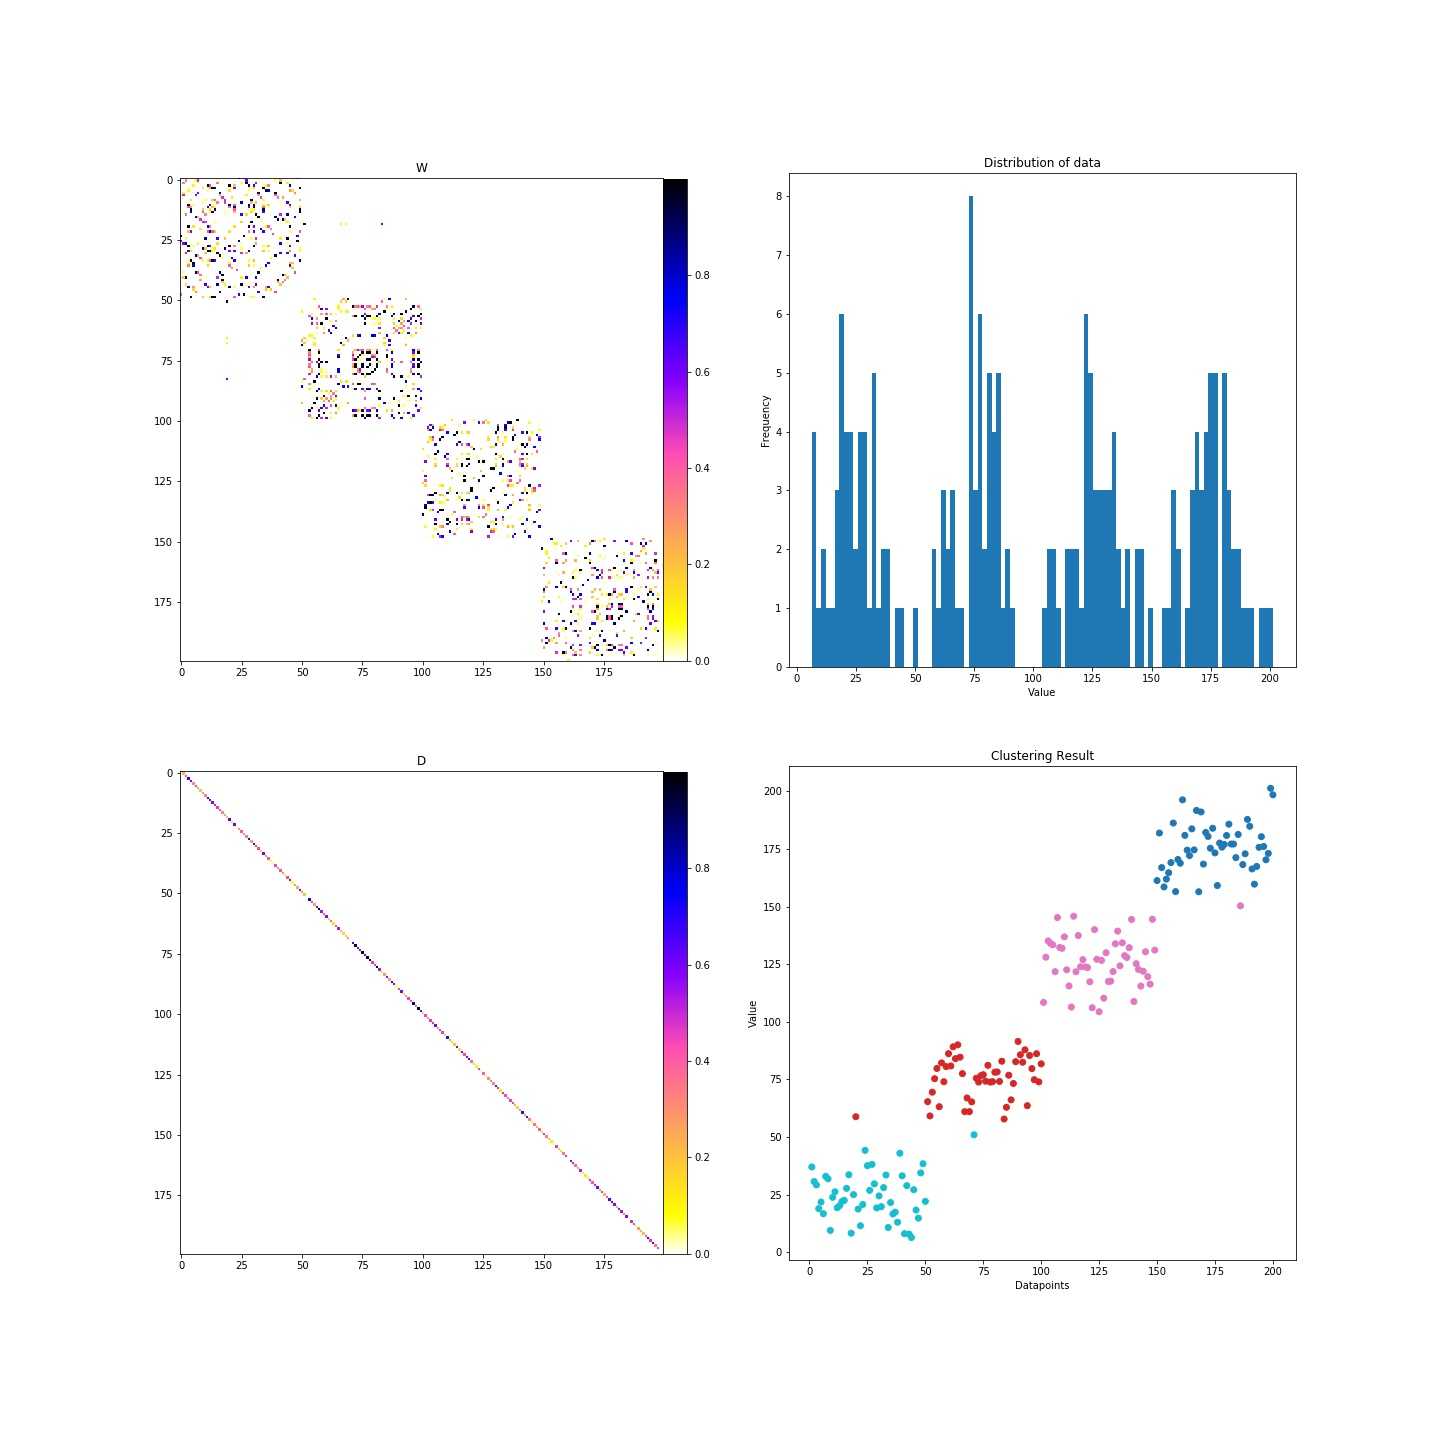
\includegraphics[height=0.80\textheight,trim=0 150 0 150,clip]{../../images/1DCluster.jpg}
			\label{fig:1dresults}
		\end{figure}
		
	\end{frame}
	
	\begin{frame}{Numerical Experiments}
		\framesubtitle{1351 Points in $\mathbb{R}^2$. Similarity function: $\lvert\lvert x-y \rvert\rvert_2^{-1}$}
		
		\begin{figure}[h]
			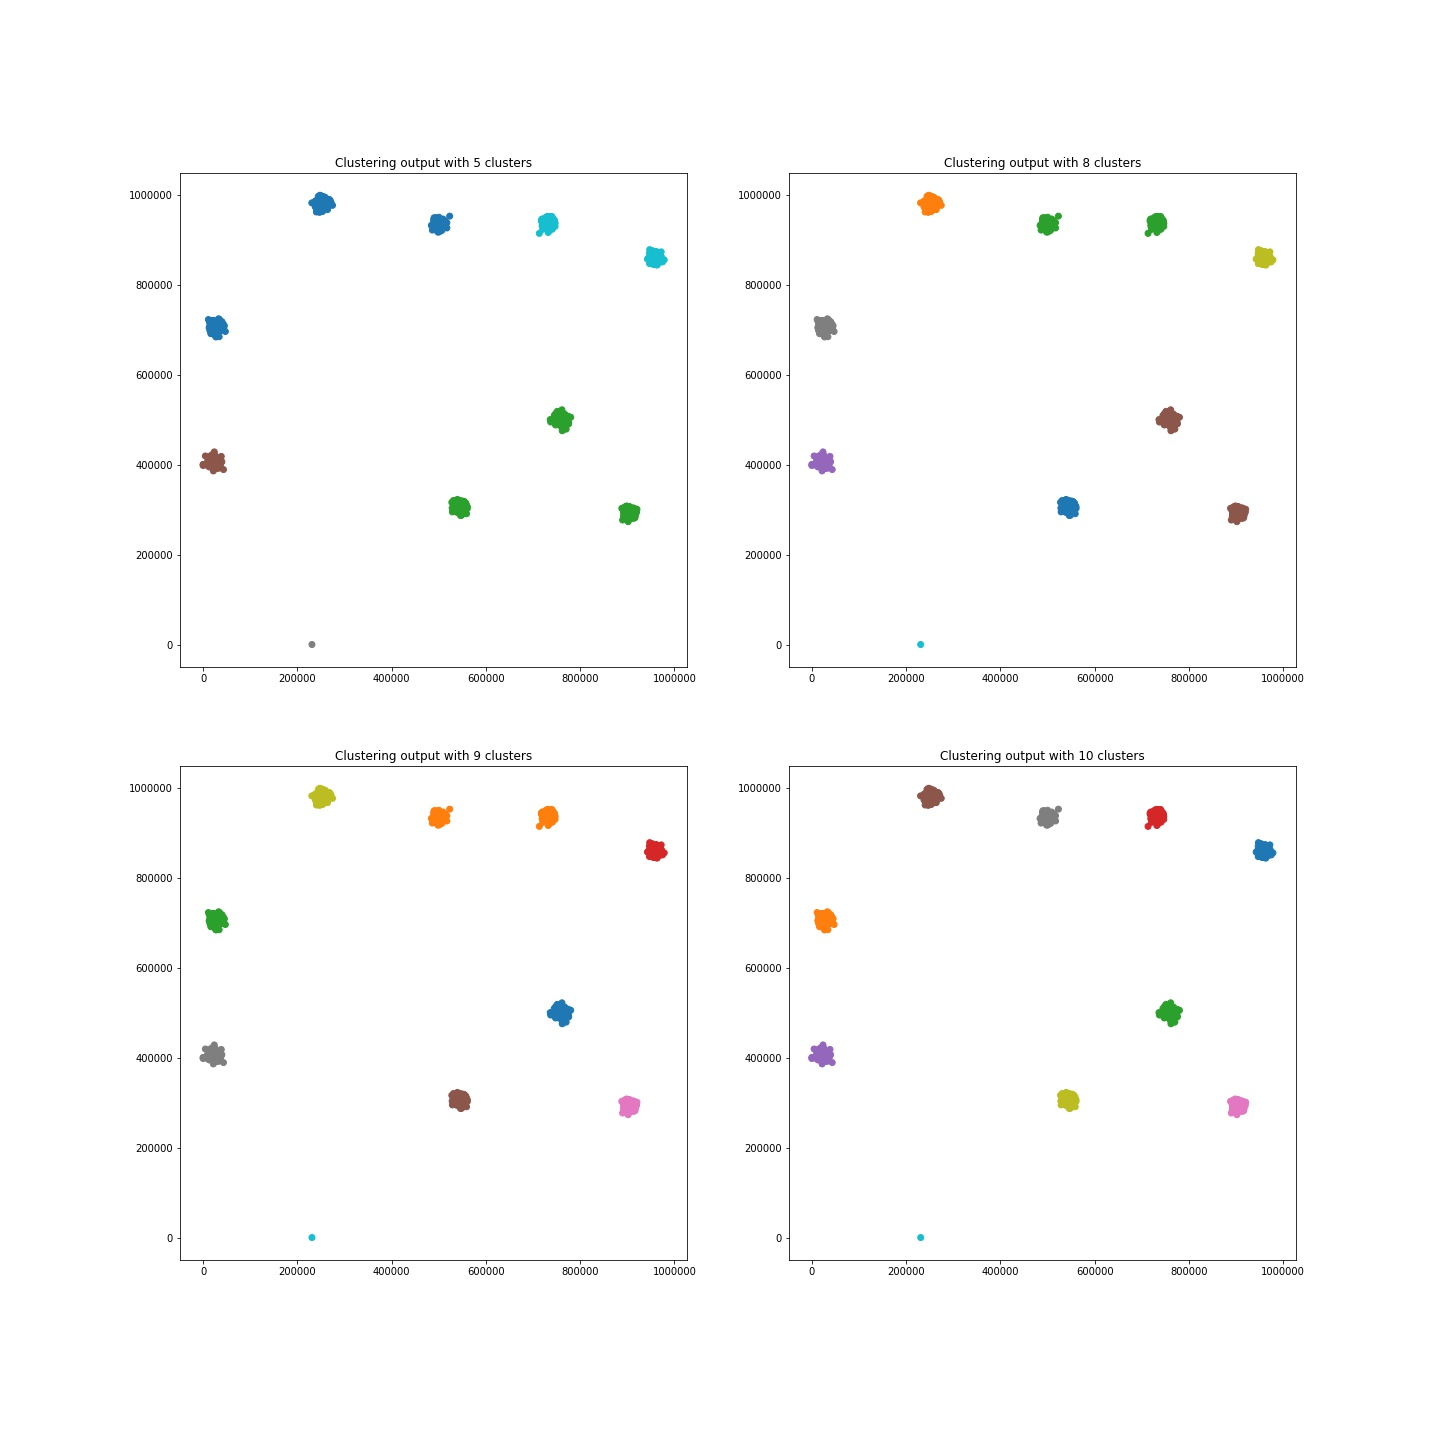
\includegraphics[height=0.80\textheight,trim=0 150 0 150,clip]{../../images/2DCluster.jpg}
			\label{fig:2dresults}
		\end{figure}
	\end{frame}
	
	\begin{frame}{Numerical Experiments}
		\framesubtitle{Image Classification. Similarity function: $\lvert \lvert \mathbf{v_i} \circ \mathbf{v_j} \rvert \rvert_1$}
		\begin{figure}[h]
			\begin{center}
				\begin{subfigure}[b]{0.45\textwidth}
					\centering
					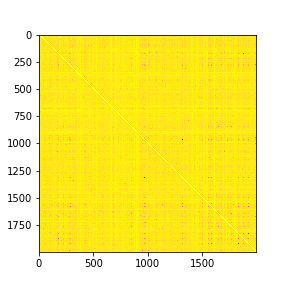
\includegraphics[width=\textwidth]{../../images/w_0norm.png}
					\caption{Weighted Adjacency Matrix}
					\label{fig:w_0norm}
				\end{subfigure}           
				\begin{subfigure}[b]{0.45\textwidth}
					\centering
					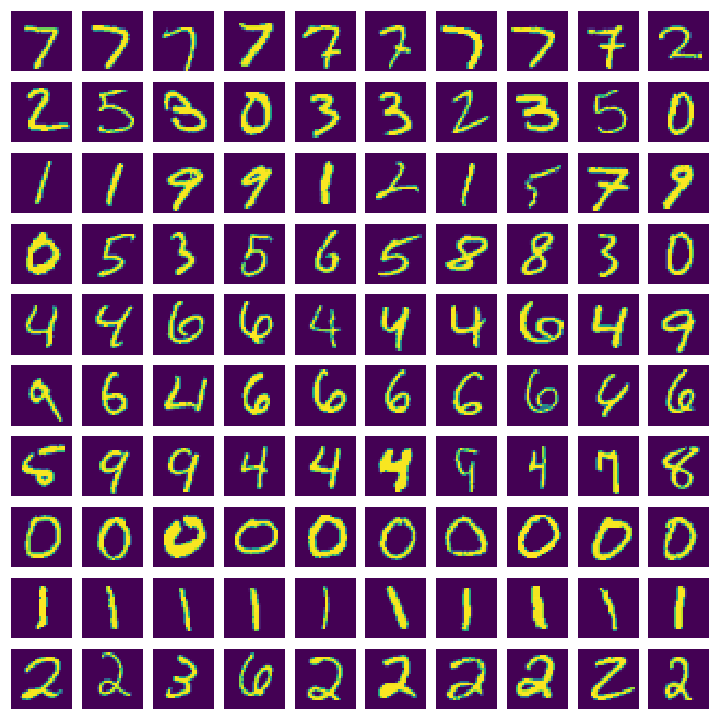
\includegraphics[width=\textwidth]{../../images/number_clustering_10_0norm.png}
					\caption{Clustering Result}
					\label{fig:clustering_10_0norm}
				\end{subfigure}           
			\end{center}
			\caption{2000 images from MNIST data-set were clustered into 10 clusters. (b) shows first 10 images in each cluster with one row per cluster}
			\label{fig:mnist10ClusterImages_1}
		\end{figure}
		
	\end{frame}
	
	
	\begin{frame}{Numerical Experiments}
		\framesubtitle{Image Classification. Similarity function: $\lvert \lvert \mathbf{v_i} - \mathbf{v_j} \rvert \rvert_2^{-1}$}
		\begin{figure}[h]
			\begin{center}

				\begin{subfigure}[b]{0.45\textwidth}
					\centering
					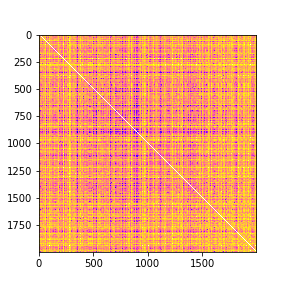
\includegraphics[width=\textwidth]{../../images/w_2norm.png}
					\caption{Weighted Adjacency Matrix}
					\label{fig:w_2norm}
				\end{subfigure}           
				\begin{subfigure}[b]{0.45\textwidth}
					\centering
					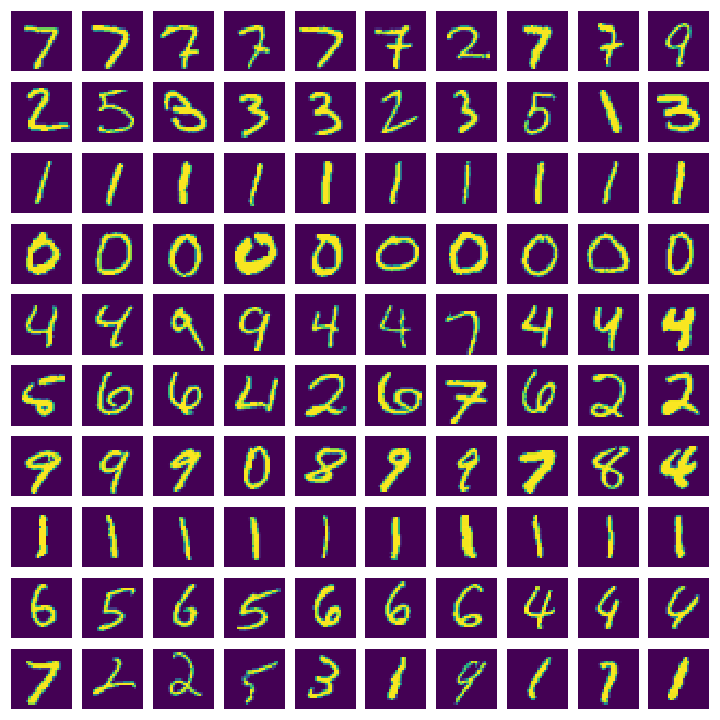
\includegraphics[width=\textwidth]{../../images/number_clustering_10_2norm.png}
					\caption{Clustering Result}
					\label{fig:clustering_10_2norm}
				\end{subfigure}           

			\end{center}
			\caption{2000 images from MNIST data-set were clustered into 10 clusters. (b) shows first 10 images in each cluster with one row per cluster}
			\label{fig:mnistWImages2}
		\end{figure}
		
	\end{frame}
	
	\begin{frame}{Numerical Experiments}
		\framesubtitle{Image Classification. Similarity function: number of pixels that either 0 or non-zero in both $\mathbf{v_i}$ \& $\mathbf{v_j}$}
		\begin{figure}[h]
			\begin{center}

				\begin{subfigure}[b]{0.45\textwidth}
					\centering
					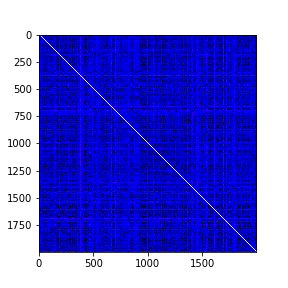
\includegraphics[width=\textwidth]{../../images/w_hamming.png}
					\caption{Weighted Adjacency Matrix}
					\label{fig:w_hamming}
				\end{subfigure}           
				\begin{subfigure}[b]{0.45\textwidth}
					\centering
					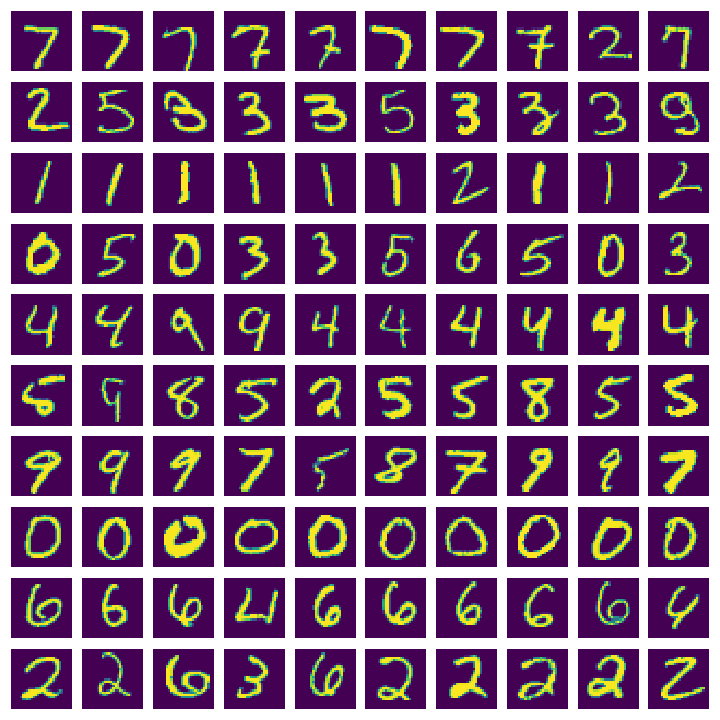
\includegraphics[width=\textwidth]{../../images/number_clustering_10_hamming.png}
					\caption{Clustering Result}
					\label{fig:clustering_10_hamming}
				\end{subfigure}           
			\end{center}
			\caption{2000 images from MNIST data-set were clustered into 10 clusters. (b) shows first 10 images in each cluster with one row per cluster}
			\label{fig:mnistWImages3}
		\end{figure}
		
	\end{frame}
	
	\begin{frame}{Numerical Experiments}
		\framesubtitle{Image Classification. Doubling the number of clusters to capture handwriting style differences}
		\begin{figure}[h]
			\begin{center}
				\begin{subfigure}[b]{0.4\textwidth}
					\centering
					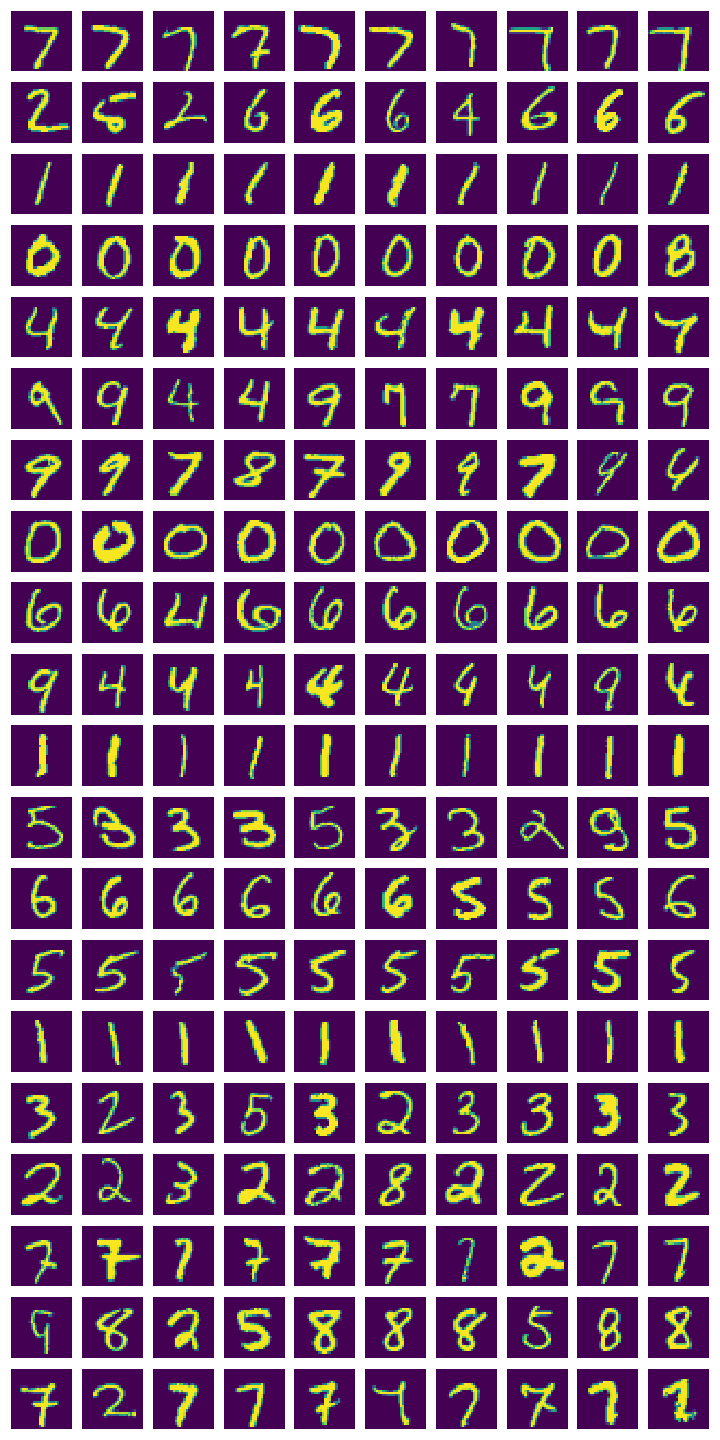
\includegraphics[height={0.6\textheight}]{../../images/number_clustering.png}
					\caption{Similarity function: $\lvert \lvert \mathbf{v_i} \circ \mathbf{v_j} \rvert \rvert_1$}
					\label{fig:clustering_20_0norm}
				\end{subfigure}
				\begin{subfigure}[b]{0.4\textwidth}
					\centering
					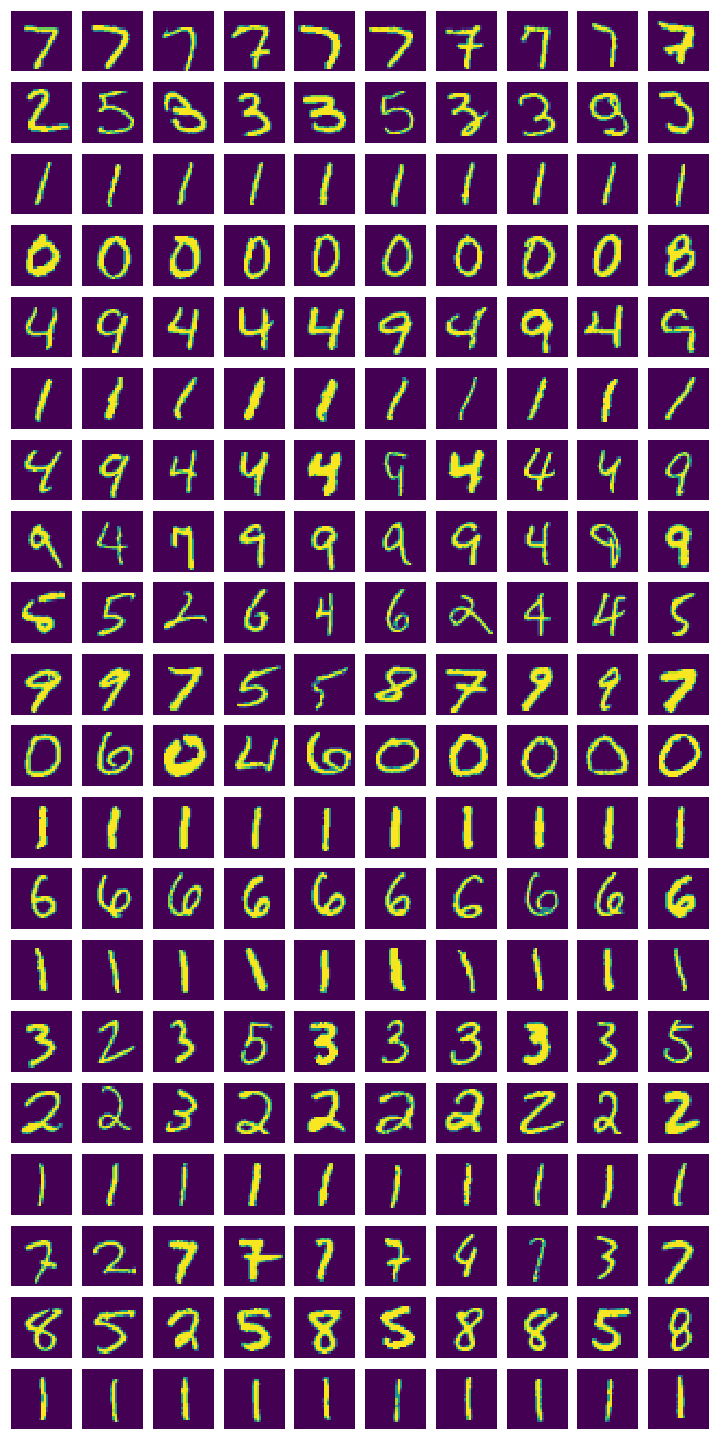
\includegraphics[height={0.6\textheight}]{../../images/number_clustering_20_2norm.png}
					\caption{Similarity function: $\lvert \lvert \mathbf{v_i} - \mathbf{v_j} \rvert \rvert_2^{-1}$}
					\label{fig:clustering_20_2norm}
				\end{subfigure}
			\end{center}
			\caption{2000 images from MNIST data-set were clustered into 20 clusters, showing first 10 images in each cluster with one row per cluster. }
			\label{fig:mnistImages}
		\end{figure}
	\end{frame}
	
	\begin{frame}{Compressive Spectral Clustering}
		\framesubtitle{[Tremblay et al. 2016]}
		Challenges with Spectral Clustering: Eigenvector computation, Cold-restart, expensive $k$-means due to high dimensionality.
		\begin{itemize}
			\item<2-> Sample $\mathcal{O}(\log(k))$ randomly filtered signals on the graph to serve as feature vectors instead of eigenvectors
			\begin{itemize}
				\item Estimate $k^{th}$ eigenvalue per [Napoli 2013	]
				\item Approximate the action of a low-pass filter $H$ that selects the first $k$ eigenvectors on the graph Laplacian
				\item Generate $\mathcal{O}(\log(k))$ Gaussian signals, filtered by $H$ to generate feature vectors $\mathbf{f_i}$
			\end{itemize}
			\item<3-> Clustering random subset of $\mathcal{O}(k\log(k))$ nodes using random feature vectors 
			\item<4-> Infer the cluster label of all $N$ nodes by interpolating. 
		\end{itemize}
		
	\end{frame}

	\begin{frame}{Future Work}
		\begin{itemize}
			\item Accelerated Eigensolvers
			\begin{itemize}
				\item Accelerating Lanczos
				\item Chebyshev-Davidson Methods	 [Zhou \& Saad 2007] [Z. Wang, 2015]
				\item Taking advantage of structure				
			\end{itemize}
			\item Detecting number of clusters adaptively.
			\item Hot-restart information from the pass with $k$ clusters to bootstrap clustering process with $k+l$ clusters 
			\item Dimensionality reduction for $k$-means
		\end{itemize}
	\end{frame}
	
	\begin{frame}
		\centering
		Thank You!
		
	\end{frame}
	 

\end{document}